\begin{figure}[htb] % 誘電関数のグラフ(lorentz+debye)
\captionsetup[subfigure]{font={bf,large}, skip=1pt, margin=-0.7cm,justification=raggedright, singlelinecheck=false}
\centering
\begin{subcaptionblock}{0.45\linewidth}
\subcaption{}\label{Fig:lorentz}
\adjustbox{right}{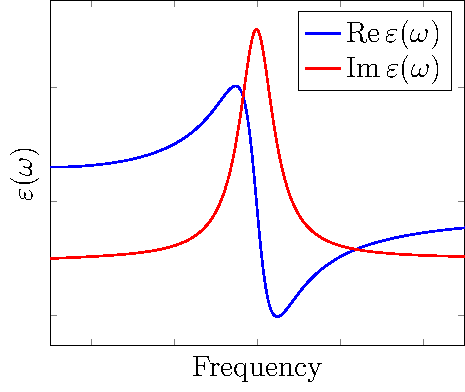
\includegraphics[width=\textwidth]{fig_1_3_lorentz/diel_lorentz.pdf}}
\end{subcaptionblock}\hfill
 \begin{subcaptionblock}{0.45\linewidth}
\subcaption{}\label{Fig:debye}
\adjustbox{right}{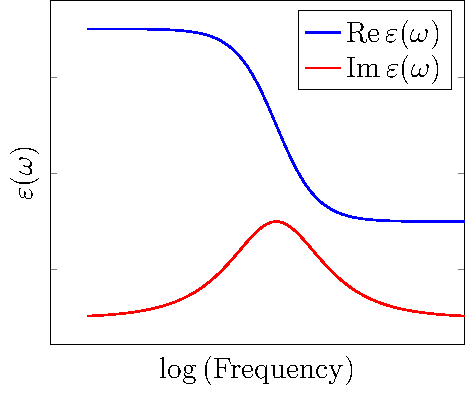
\includegraphics[width=\textwidth]{fig_1_3_lorentz/diel_debye.pdf}}
\end{subcaptionblock}
  \caption{The typical dielectric function of (a) the Lorentz model and (b) the Debye model. The blue lines represent the real part of the dielectric function, while the red lines correspond to the imaginary part. The peak positions of the imaginary part of the dielectric function are given by the resonance frequency $\omega_{0}$ and the inverse of the relaxation time $1/\tau$ for the Lorentz and Debye models, respectively.}
\label{Fig:models}  
\end{figure}

